\section{Experimental Evaluation}
\subsection{Dataset Description}
We collected crowdsourced segmentations from Amazon Mechanical Turk where each HIT consisted of one segmentation task for a specific pre-labeled object in the image. There were a total of 46 objects in 9 images from the MSCOCO dataset~\cite{Lin2014}. For each object, we collected segmentation masks from a total of 40 workers. Each task contains a semantic keyword and a pointer indicating the object to be segmented. %These tasks represent a diverse set of task difficulty (different levels of clutteredness, occlusion, lighting) and levels of task ambiguity. 
\subsection{Evaluation Metrics}
\par Evaluation metrics used in our experiment measures how well the final segmentation (S) produced by these algorithms compare against ground truth (GT). The most common evaluation metric used in literature are area-based methods which take into account the intersection, $IA=area(S\cap GT)$, or union, $UA=area(S\cup GT)$, between the user and the ground truth segmentations. Specifically, we use
    $\text{Precision (P)} = \frac{IA(S)}{area(S)}$, 
    $\text{Recall (R)} = \frac{IA(S)}{area(GT)}$, and 
    $\text{Jaccard (J)} = \frac{UA(S)}{IA(S)}$
    metrics to evaluate our algorithms.
 \techreport{\par A sub-sampled dataset was created from the full dataset to determine the efficacy of these algorithms on varying number of worker responses. Every object was randomly sampled worker with replacement. For small worker samples, we average our results over larger number of batches than for large worker samples (which have lower variance, since the sample size is close to the original data size).}
 \subsection{Evaluation Results}
 \stitle{Aggregation-based methods performs significantly better than retrieval-based methods}
\par \noindent Figure~\ref{retrieval_vs_aggregation} left shows that amongst the algorithms that do not make use of ground truth information, the performance of aggregation-based algorithms (greedy, EM) exceeds the best achievable through the existing retrieval-based method (num pts). By making use of ground truth information (Figure~\ref{retrieval_vs_aggregation} right), the best aggregation-based algorithm can achieve a close-to-perfect average Jaccard score of 0.98 as an upper bound, far exceeding the results achievable by any single `best' worker (J=0.91). This result demonstrates that aggregation-based methods are able to achieve better performance by performing inference at the \textit{tile} granularity, which is guaranteed to be finer than any individual worker segmentation. 
\begin{figure}[h!]
   \vspace{-10pt}
   \centering
   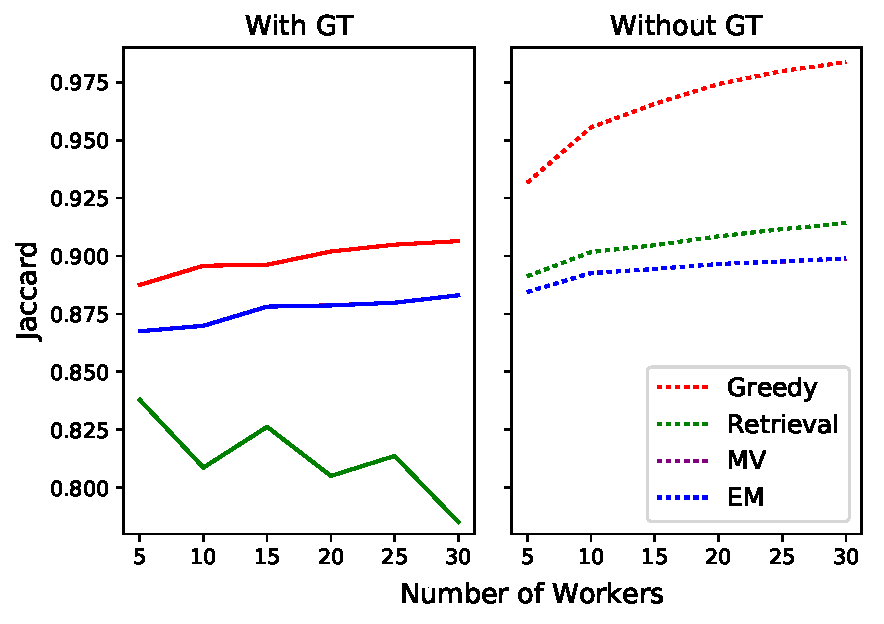
\includegraphics[width=0.9\textwidth]{plots/Retrieval_vs_Aggregation.pdf}
   \caption{Jaccard performance comparison between best-performing algorithms from retrieval and aggregation-based methods with clustering as a preprocessing step where possible. We compare between the original algorithms that do not make use of ground truth information (Left) and ones that do (Right). Note that MV and EM results are so close that they overlay on each other.}
   \label{retrieval_vs_aggregation}   
\end{figure} 
% \vspace{-10pt}

\stitle{Performance of aggregation-based methods scales well as more workers segmentation are added.}
\par \noindent Intuitively, larger worker samples results in finer granularity tiles for the aggregation-based methods, resulting in an monotonically increasing relationship between number of worker segmentation used in the sample and performance evident in Table~\ref{statsTable}. However, worker scaling for retrieval-based methods are not guaranteed.

\stitle{Clustering as preprocessing improves algorithmic performance.}
\par \noindent As shown in Table~\ref{statsTable}, on average, clustering generally results in an increase the resulting algorithmic performance. Since the ground-truth supervised variants are already free of semantic ambiguity and errors, there is minimal improvement resulting from clustering. %In particular, we see a greater improvement with clustering preprocessing for algorithms that are not very robust in resolving semantic errors or ambiguity, such as for the \texttt{num pts} retrieval algorithm, than compared to the aggregation-based methods. 

\begin{table}[h!]
   \small
     \setlength\tabcolsep{1.5pt}
      \begin{tabular}{l|l|l|l|l|l|l}
         & \multicolumn{2}{c|}{Retrieval-based} & \multicolumn{4}{l}{Aggregation-based} \\ \hline
      Algorithm         & num pts         & worker*        & MV    & EM    & greedy  & greedy*  \\ \hline
      Worker Scaling    & -6.30           & 2.58               & 1.63  & 1.64  & 2.16    & 5.59         \\ \hline
      Clustering Effect & 5.92            & -0.02              & 2.05  & 1.38  & 5.55    & -0.06       
      \end{tabular}
      \caption{The first row lists the average percentage change in Jaccard between 5 workers samples and 30 workers sample. The second row lists the average percentage change between the no clustering and clustering results. Algorithms with * makes use of ground truth information.}
      \label{statsTable}
\end{table}
\vspace{-10pt}
